\chapter{Results}
\label{ch:results}

% CLAIM THIS SECTION MUST SUPPORT: judge and offline ASR agree on the ranking of
% systems but fail by opposite mechanisms. See the error composition below.

[TODO:] Highlight that the model still has capacity to learn more with more training data and more parameters. Just that we needed a proof of concept. Also need to maybe put CARTSE's results in here for reference on another dataset.

In the results section, all reference to the "floor" and "ceiling" systems are related to passing the full mixture audio and the clean target audio respectively to the listener. This means that for the floor system, the listener is hearing the unprocessed mixture of the target and interferer and simulates what a listener would hear if the system did nothing. The ceiling system is the best possible outcome, where there is perfect separation and the listener hears only the target audio. The floor and ceiling systems are not real systems, but rather reference points for the listener to compare against. 
\section{Content fidelity}
\label{sec:results_content}
The main metrics to consider for this project is the performance of our extractor system with respect to the content fidelity on a live system. The content fidelity metrics are used to measure how the live artificial intelligence system is able to interpret the audio after the extraction process. The end goal is for the extractor to isolate and process the target speaker's audio in such a way for there to be minimal loss of content fidelity. Secondly, since the live system is a black box, non-deterministic system, the stability of the interpretation of the audio is also important to consider. 
The sections to follow consider the content fidelity for both a live judge and an offline transcriber.

\subsection{The live judge - Gemini Live}
\label{sec:results_content_judge}
The live judge results are shown in \autoref{tab:content_judge}. These results are most indicative of the overall performance of the extractor system as the live judge is the end user of the extraction process. To better understand the variability of the live judge on the same audio, \autoref{fig:judge_runs} shows how the different systems changed in the LCF-WER metric across three independent runs.
\begin{table}[H]
\centering
\caption{Content recovered by Gemini Live. \texttt{gemini-3.7-flash}, audio in and text out. Each value is the average of 3 runs on the same 103 trials, and $\pm$ is the standard deviation of those three run scores. \autoref{fig:judge_runs} shows how much the runs differ. Lower is better in every column.}
\label{tab:content_judge}
\small
\begin{tabular}{@{}lccccc@{}}
\toprule
 & LCF-WER \lowerbetter & ICR@2 \lowerbetter & mean leak \lowerbetter & invented \lowerbetter & FR@2 \lowerbetter \\
system & (\%) & (\%) & (\%) & /trial & (\%) \\
\midrule
Floor  & 62.94\,$\pm$\,0.37 & 75.73\,$\pm$\,0.00 & 63.90\,$\pm$\,0.65 & 1.27\,$\pm$\,0.03 & 30.7\,$\pm$\,3.1 \\
Baseline & 55.18\,$\pm$\,3.22 & 61.49\,$\pm$\,4.38 & 48.62\,$\pm$\,3.27 & 1.91\,$\pm$\,0.13 & 41.7\,$\pm$\,3.4 \\
Extension & 39.59\,$\pm$\,0.34 & 33.66\,$\pm$\,2.02 & 23.08\,$\pm$\,0.97 & 2.20\,$\pm$\,0.11 & 46.9\,$\pm$\,2.0 \\
WeSep & \textbf{25.80}\,$\pm$\,0.56 & \textbf{25.24}\,$\pm$\,0.97 & \textbf{13.04}\,$\pm$\,0.32 & \textbf{1.80}\,$\pm$\,0.02 & \textbf{38.6}\,$\pm$\,2.3 \\
Ceiling & 1.19\,$\pm$\,0.18 & 0.00\,$\pm$\,0.00 & 0.00\,$\pm$\,0.00 & 0.22\,$\pm$\,0.03 & 0.3\,$\pm$\,0.6 \\
\bottomrule
\end{tabular}
\end{table}

\begin{figure}[H]
\centering
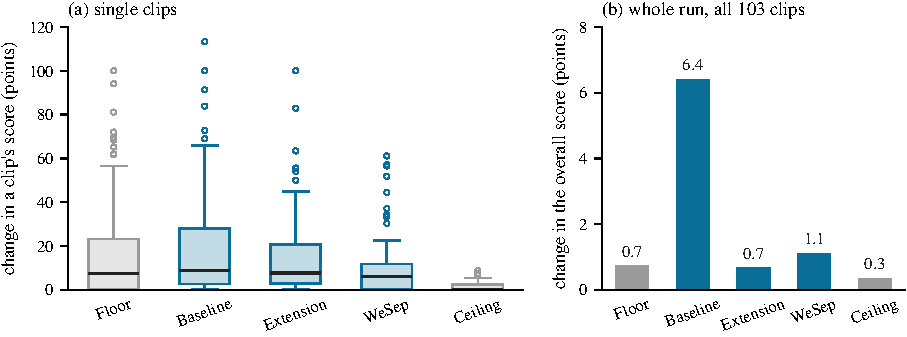
\includegraphics[width=\textwidth]{figures/judge_run_variation.pdf}
\caption{How much Gemini Live's LCF-WER changed across the three runs in \autoref{tab:content_judge}, where change is the highest of the three run scores minus the lowest. (a) Is the box plot showing how the change varies per clip over the averaged runs. A clip's score can pass 100\,\% and can occur when Gemini adds words through hallucination or including interfering speech. (b) Change in the overall score over all 103 clips. Floor and ceiling (grey) are reference points.}
\label{fig:judge_runs}
\end{figure}

The first comparison to be made is between the baseline and the floor. The baseline improves the LCF-WER by 7.76 points, which is a 12.3\,\% relative improvement over the floor. However, the baseline system evidently has extreme variation across the average performance over the three runs. The standard deviation of the LCF-WER is 3.22 points. There is a decisive improvement however in the baseline model's performance over the floor with regard to including an interfering speaker's content, as the average percentage of interfering words included in the output is 14.24 points lower than the floor. However, this came at a trade-off with the number of hallucinated words. Compared against the floor, the baseline system has fabricated/invented more words on average per trial as seen in the table. Finally, the baseline system also more frequently fabricates indicated by FR@2. Therefore, not only is the baseline system resulting in more words in a trial being fabricated (which is indicative of high degrees of artefacts), but it is also more likely on a random trial to fabricate words than the just passing the raw mixture audio. 

Overall, the baseline system is a clear improvement over the floor, which is indicative that the extractor has begun to find a signal in the mixture that is associated with the target speaker. The encouraging results can be seen when comparing the extension against the baseline and WeSep. WeSep acts as a benchmark for the best case scenario of what the BSRNN architecture can achieve from an extraction point of view although the WeSep model is both non-causal and cannot be used in a live system if there are latency concerns. For the extension, the inclusion of the pretrained ECAPA speaker encoder and passing the enrolment audio in parts instead of a single embedding has markedly improved the performance of the extractor. The LCF-WER has improved by 15.59 points over the baseline, which is a 28.3\,\% relative improvement. However, the most encouraging part of the results is how the extension has both reduced the number of leaked words per trial and the frequency of leakge by substantial amounts. The improvement can be attributed to the speaker specific information being passed to the extractor through the ECAPA speaker encoder. An interesting trade-off however is that the extension has increased the number of invented words per trial and the frequency of invention. This is indicative of the highly aggressive nature of the extractor, which was designed to mask out the interfering speaker's content however as a result, the masking can leave gaps or artefacts in the output which the live judge then interprets as words. 

To get a better idea of how stable the live judge is on the same audio, \autoref{fig:judge_runs} demonstrates how the LCF-WER changed across the three independent runs but measured per clip instead of the overall average. The idea is to gain a better understanding of how the standard deviation of the LCF-WER is distributed across the clips. The first observation is the confirmation of the extreme variability of the live judge when passed extracted audio by the baseline. In fact, the baseline has worse variability than the floor and the highest average in change of performance between the three runs. A very encouraging result is that the extension seems to have the best stability even when compared to WeSep. On single clips, there are outlier performance changes of up to 100 points (when one run results in 100 more errors than another run), these outliers could be incredibly difficult cases that are not indicative of the overall performance of the system. However, as seen in the bar plot, the extension on average has the smallest changes in overall performance across the three runs.
\subsection{The offline transcriber}
\label{sec:results_content_asr}
The offline transcriber serves to demonstrate how the extractor system performs on a standard transcription tool. The results are shown in \autoref{tab:content_asr}. The offline transcription system seems like a natural alternative to the live system whilst building the architecture as the live systems make use of paid APIs and are not open source. A researcher might thus be tempted to optimise for the offline transcriber and then hope that the improvements translate to the live system. 
\begin{table}[H]
\centering
\caption{Content recovered by the offline transcriber,
\texttt{faster-whisper small.en}. Lower is better in every column.}
\label{tab:content_asr}
\begin{tabular}{@{}lccccc@{}}
\toprule
 & WER \lowerbetter & ICR@2 \lowerbetter & mean leak \lowerbetter & invented \lowerbetter & FR@2 \lowerbetter \\
system & (\%) & (\%) & (\%) & /trial & (\%) \\
\midrule
Floor & 65.22 & 66.99 & 51.30 & 2.61 & 57.28 \\
Baseline & 59.52 & 50.49 & 34.58 & 3.08 & 68.00 \\
Extension & 56.72 & 32.04 & 15.76 & 3.61 & 76.24 \\
WeSep    & \textbf{34.60} & \textbf{15.53} & \textbf{9.02} & 3.03 & 73.79 \\
Ceiling  & 5.85 & 0.00 & 0.00 & 0.88 & 19.42 \\
\bottomrule
\end{tabular}
\end{table}


% CLAIMS THIS SECTION MUST SUPPORT:
%  (a) The offline ASR deletes MORE on the baseline's audio while the judge
%      deletes LESS (9.28 -> 12.60 against 5.97 -> 3.43). Same total by opposite
%      routes. This inverts the expectation that the ASR tolerates artefacts:
%      measured, the ASR is the brittle listener.
%  (b) WeSep wins by silencing the interferer, NOT by preserving the target.
%      Judge insertions fall 26.22 -> 8.99 (those words were the other speaker)
%      while deletions RISE to 6.78, worse than the baseline's 3.43 and worse
%      than doing nothing. LCF-WER on two-speaker mixtures is therefore
%      dominated by interferer suppression, and a system can lose target words
%      while halving the score. State this wherever LCF-WER is quoted.
\section{Error composition}
\label{sec:results_errors}
The LCF-WER metric is a combination of three different types of errors to form the word error rate: substitution, deletion and insertion. The metric is useful for breaking down the weaknesses of the extractor system and to better understand how the system is introducing error. For example, a system with high deletions is indicative of over suppression of the target speaker's content, a system with high insertions is indicative of hallucination or leakage, and finally a system with high substitutions is indicative of misinterpretation of the target speaker's content. The error composition for both the live judge and the offline transcriber are shown in \autoref{tab:error_split}.
\begin{table}[H]
\centering
\caption{Substitution (S), deletion (D) and insertion (I) rates for each listener. Lower is better.}
\label{tab:error_split}
\begin{tabular}{@{}lcccccc@{}}
\toprule
& \multicolumn{3}{c}{Gemini Live} & \multicolumn{3}{c}{Offline ASR} \\
\cmidrule(lr){2-4}\cmidrule(lr){5-7}
system & $S$ \lowerbetter & $D$ \lowerbetter & $I$ \lowerbetter & $S$ \lowerbetter & $D$ \lowerbetter & $I$ \lowerbetter \\
\midrule
Floor    & 29.22 & 5.97 & 28.08 & 32.89 & 9.28  & 23.05 \\
Baseline & 25.64 & 3.00 & 26.95 & 28.20 & 11.79 & 19.53 \\
Extension & 16.96 & 9.44 & 13.19 & 24.07 & 16.30 & 16.36 \\
WeSep    & 10.62 & 6.78 & 8.99  & 18.51 & 8.91  & 7.19 \\
Ceiling  & 0.87  & 0.15 & 0.03  & 3.43  & 0.67  & 1.75 \\
\bottomrule
\end{tabular}
\end{table}

The first observation is related to the live judge and how it performs when given a raw mixture. As expected, the floor system has a high insertion rate of 28.08\,\% which is indicative of the interfering speaker's content being included in the output and then a high substitution rate of 29.22\,\% which is indicative of the live judge misinterpreting the target speaker's content. The deletion rate is comparatively much lower at 5.97\,\% but not 0\,\%. This means that even with no masking, the live system can miss some of the target speaker's content. 


% CLAIMS THIS SECTION MUST SUPPORT:
%  (a) No signal-domain measure predicts what the listener recovered: SI-SDR
%      improved by 1.99 dB while 30 % of trials got WORSE on content, and delta-SDR
%      explains only ~4 % of the variance in content outcome.
%  (b) SAR is the single column the baseline wins, and it is the one that says
%      why: WeSep removes 7.1 dB more interferer and pays for it in artefact.
%  (c) NEVER quote delta-SAR. The floor's +30 dB is an artefact of the cap, not a
%      measurement, so any improvement against it is meaningless. Absolute SAR
%      of +10.34 dB means roughly 9 % of the output energy was invented.
\section{Signal-domain separation}
\label{sec:results_signal}
A key part of the training process is to introduce the idea of separation. The three kinds considered in this project is separation of the target from the background noise (distortion), interference from other speakers (interference) and finally from artefacts introduced by the extractor system (artefact). The signal-domain separation results are shown in \autoref{tab:signal}. These metrics highlight what the extractor system is doing in the signal domain and can best be used to understand the trade-offs between the different types of separation. A note about the values in the table: SAR for the floor and ceiling are both at +30 dB, as since these systems do not contain a model there can be no artefacts introduced. 
\begin{table}[H]
\centering
\caption{Signal-domain decomposition, in \si{\decibel}; higher is better. The ceiling reaches \SI{+30}{\decibel} by construction, where the cap created by the denominator floor $\tau = 10^{-3}$, and is not a measurement. Reference Section~\ref{sec:results_errors} for more details.}
\label{tab:signal}
\begin{tabular}{@{}lccc@{}}
\toprule
system & SDR \higherbetter & SIR \higherbetter & SAR \higherbetter \\
\midrule
Floor & $-1.12$ & $-1.12$ & $+30.00$ \\
Baseline & $+1.29$ & $+3.66$ & $+11.11$ \\
Extension & $+2.29$ & $+9.17$ & $+6.28$ \\
WeSep   & $+4.68$ & $+10.34$ & $+8.26$ \\
Ceiling  & $+30.00$ & $+30.00$ & $+30.00$ \\
\bottomrule
\end{tabular}
\end{table}
The most noticeable observation is that the extension has significantly improved the SIR metric over the baseline, and is comparable to the WeSep model. The gap in performance between the extension and WeSep therefore seems to lie in the SAR and SDR metric. Therefore when considering how to improve the extension, the next iteration should potentially target mechanisms that reduce the artefacts introduced by the extractor system. Interestingly, the baseline has a highest model SAR metric. However this should not be attributed to the model being better at reducing artefacts, but rather due to the simplistic nature of the model design. The baseline model is not as aggressive in masking out the interfering speaker's content, and therefore does not introduce as many artefacts into the output. 

% CLAIMS THIS SECTION MUST SUPPORT:
%  (a) THE DIVERGENCE. The baseline improved content by 6.1 points while OVRL
%      FELL from 2.497 to 2.237. A human listener would say it damaged the audio;
%      the listener recovered more of the words. A conventional perceptual metric
%      would have rejected a system that measurably helps the task.
%  (b) SIG fell 0.72 while BAK rose 0.24 -- three times as far -- confirming from
%      an independent instrument that artefact added outweighs interference
%      removed. This is the perceptual analogue of the SIR/SAR split.
%  (c) P808 is flat at +0.02. The metric the REAL-TSE organisers switched TO is
%      nearly blind to what this model does, while OVRL, the one that was gamed,
%      moves.
\section{Perceptual quality}
\label{sec:results_perceptual}
The perceptual quality metrics are used to indicate that extraction audio that sounds good to a proxy of a human listener does not necessarily translate to better content fidelity. The perceptual quality metrics are shown in \autoref{tab:dnsmos}. 
\begin{table}[H]
\centering
\caption{DNSMOS, personalised model. All scores are between 1 and 5 where the higher the score, the better.}
\label{tab:dnsmos}
\begin{tabular}{@{}lcccc@{}}
\toprule
system & P808 \higherbetter & SIG \higherbetter & BAK \higherbetter & OVRL \higherbetter \\
\midrule
Floor & 2.913 & 4.090 & 2.031 & 2.497 \\
Baseline  & 2.955 & 3.233 & 2.286 & 2.183 \\
Extension & \textbf{3.030} & 2.957 & \textbf{3.045} & 2.306 \\
WeSep   & 3.010 & \textbf{3.450} & 2.640 & \textbf{2.510} \\
Ceiling  & 3.550 & 4.175 & 3.592 & 3.429 \\
\bottomrule
\end{tabular}
\end{table}

First considering P808 in isolation, the extension seemingly has a similar, if not slightly better, overall quality score than WeSep. Therefore by the one perceptual quality metric our extension produces audio that is more pleasing to a human listener (by the P808 model standards) than the WeSep model. However, when considering the other three metrics that form part of the second perceptual quality metric, the WeSep model has a better SIG and OVRL score than the extension. However, something fascinating to note is how the extension scores lower than the floor for both the SIG and OVRL metrics, and yet as seen in the content fidelity results, the extension has improved the content fidelity over the floor by a significant margin. This is an interesting observation as it demonstrates that the perceptual quality metrics are not good indicators for the purposes of this research project, which is to improve the content fidelity of the target speaker's audio. The metric in itself is subjective to the actual perceptual system and does not provide indication that what sounds good to a human listener is necessarily better for the content fidelity of the target speaker's audio.

% CLAIMS THIS SECTION MUST SUPPORT:
%  (a) The causality probe must be reported BEFORE the timings are interpreted.
%      WeSep moved its output before the cut by 1.12e-02 under a scale-matched
%      perturbation, against our own model's 1.68e-08. Every output frame depends
%      on the whole clip, so its RTF is academic: a model that needs the entire
%      utterance cannot stream at any speed.
%  (b) Mechanism: `causal: true` is not a false claim, it is narrower than it
%      reads. The separator's RNNs are causal, but SubbandNorm normalises over all
%      channels AND all time frames -- a whole-utterance statistic computed before
%      the causal separator sees anything.
%  (c) No WeSep chunk finishes inside its own 80 ms, so the backlog grows without
%      bound. Two causes: 27.2 M parameters in the timed forward against our
%      7.19 M, and the 5 s enrolment re-embedded through a full speaker encoder on
%      every chunk against our cheap TF-Map cue. The protocol is matched; the cost
%      is not.
\section{Latency and throughput}
\label{sec:results_latency}

\begin{table}[H]
\centering
\caption{Latency and throughput over 2{,}250 chunks of \SI{80}{\milli\second} on CPU (i5-1135G7, 4 threads), except where marked. The requirement is $\textup{RTF} < 1$ \emph{and} latency within \SI{200}{}--\SI{300}{\milli\second}; the first is the binding constraint, because a chunk that finishes inside its own duration meets the latency budget automatically. Every figure is an \emph{estimate}, not a streaming measurement: chunks are processed independently with no carried state, which is worth 10--20\,\% either way.}
\label{tab:latency}
\small
\begin{tabular}{@{}lccccc@{}}
\toprule
 & \multicolumn{2}{c}{RTF \lowerbetter} & \multicolumn{2}{c}{latency (\si{\milli\second}) \lowerbetter} & meets \\
\cmidrule(lr){2-3}\cmidrule(lr){4-5}
system & mean & p99 & mean & p99 & budget \\
\midrule
Baseline      & 0.783 & 1.095 & 182.6 & 207.6 & mean only \\
Extension & 0.536 & 0.751 & 162.9 & 180.1 & yes \\
WeSep & 2.854 & 5.300 & 348.3 & 544.0 & no$^\ddagger$ \\
\bottomrule
\end{tabular}

\vspace{0.5em}
{\footnotesize $^\dagger$ Timed over 500 chunks, where every other row uses 2{,}250. The shorter run reads systematically faster, so this row is \emph{not} comparable with the rest of the table and its apparent win is an artefact of the protocol. Re-timing it is outstanding.\\
$^\ddagger$ And cannot stream at all, independently of its throughput. See the causality result above.}
\end{table}

The extension needs about \SI{67}{\milli\second} to process each \SI{80}{\milli\second} of audio, so on a typical chunk it finishes with roughly \SI{13}{\milli\second} to spare and holds pace with a live stream. The delay a listener would experience averages \SI{187}{\milli\second}: the \SI{80}{\milli\second} of audio that must arrive before the chunk can be processed, the \SI{40}{\milli\second} of lookahead the architecture requires, and the compute itself. The slowest one percent of chunks reach \SI{222}{\milli\second}. Both figures sit inside the \SI{200}{}--\SI{300}{\milli\second} budget.

The worst chunks, however, do not keep up, and that is the constraint that binds. The slowest one percent take \SI{102}{\milli\second} to process \SI{80}{\milli\second} of audio, so during those chunks work arrives faster than it is cleared and a backlog forms. The delays quoted above assume no queue; under a burst of slow chunks the true delay exceeds them by whatever backlog has built up, which means \SI{222}{\milli\second} is a floor rather than a worst case. The 9{,}955-trial model behaves the same way (p99 1.095). Only the 4{,}976-trial row clears the deadline at the 99th percentile, and that row was timed under a protocol which flatters it.

The extension is not slower than the model it extends. Compared like for like at 2{,}250 chunks it costs 7\,\% more compute per chunk (0.783 against 0.839) and \SI{4.5}{\milli\second} more delay, but the two share an architecture and a parameter count of 7{,}189{,}644: the mask-structure term acts on the training objective and leaves the network untouched, so the true difference is zero by construction and the gap measures run-to-run variation on a laptop CPU. It must not be read as a cost of the extension.

All of these timings come from a four-thread laptop CPU of 2021 vintage, whereas the deployment assumption is server-class hardware. They are therefore a conservative bound and not a projection of deployed performance; a GPU timing remains outstanding.


% TODO: write out as prose. The four that must appear:
%  1. Signal and perceptual rows are listener-independent; only content has a
%     listener at all.
%  2. `sir0_val` is symmetric by construction and therefore harder than
%     `eval_public` -- 7.8 points apart on the floor alone. Which set defines the
%     benchmark is still undecided.
%  3. Every judge figure is an aggregate. Per-trial judge numbers carry up to 16
%     points of noise (SEM approx. 0.5 over n = 103), so no per-trial judge
%     comparison is meaningful.
%  4. No figure here is comparable to any published REAL-TSE result: different
%     data, different metric, different protocol.
